\section{Results}
\label{sec:results}
\subsection{Do susceptibility scores predict isolated damage?}
Figure~\ref{fig:validity} compares scores with the positive part of exact
isolated loss change. The balanced-stratum associations are positive for most
methods but far from perfect. On ResNet-8, per-example absolute ranking has
Spearman correlation .376, compared with .364 for global first-order and .256
for MSB-first. Numerical jump alone is much weaker (.070). KWS has smaller
associations: .288 for per-example absolute, .258 for global first-order and
.204 for MSB-first. Overlapping candidate-bootstrap intervals do not establish
pairwise estimator superiority; the point estimates describe this sampled design.

ToyCar's positive per-example score has the strongest point association (.637),
followed by per-example absolute (.546) and MSB-first (.502). However, the measured
damage in that panel is reconstruction MSE, not ROC-AUC. It would be a category
error to infer that the best MSE association must give the best anomaly-detection
protection. The random reference's near-zero correlations are from a single
sampled ordering, not a population confidence statement about random policies.
Signed and absolute damage results, tied-score fractions and sample top-$k$
statistics are retained in the evidence supplement rather than collapsed into a
single claim of estimator quality.

\begin{figure}[t]\centering
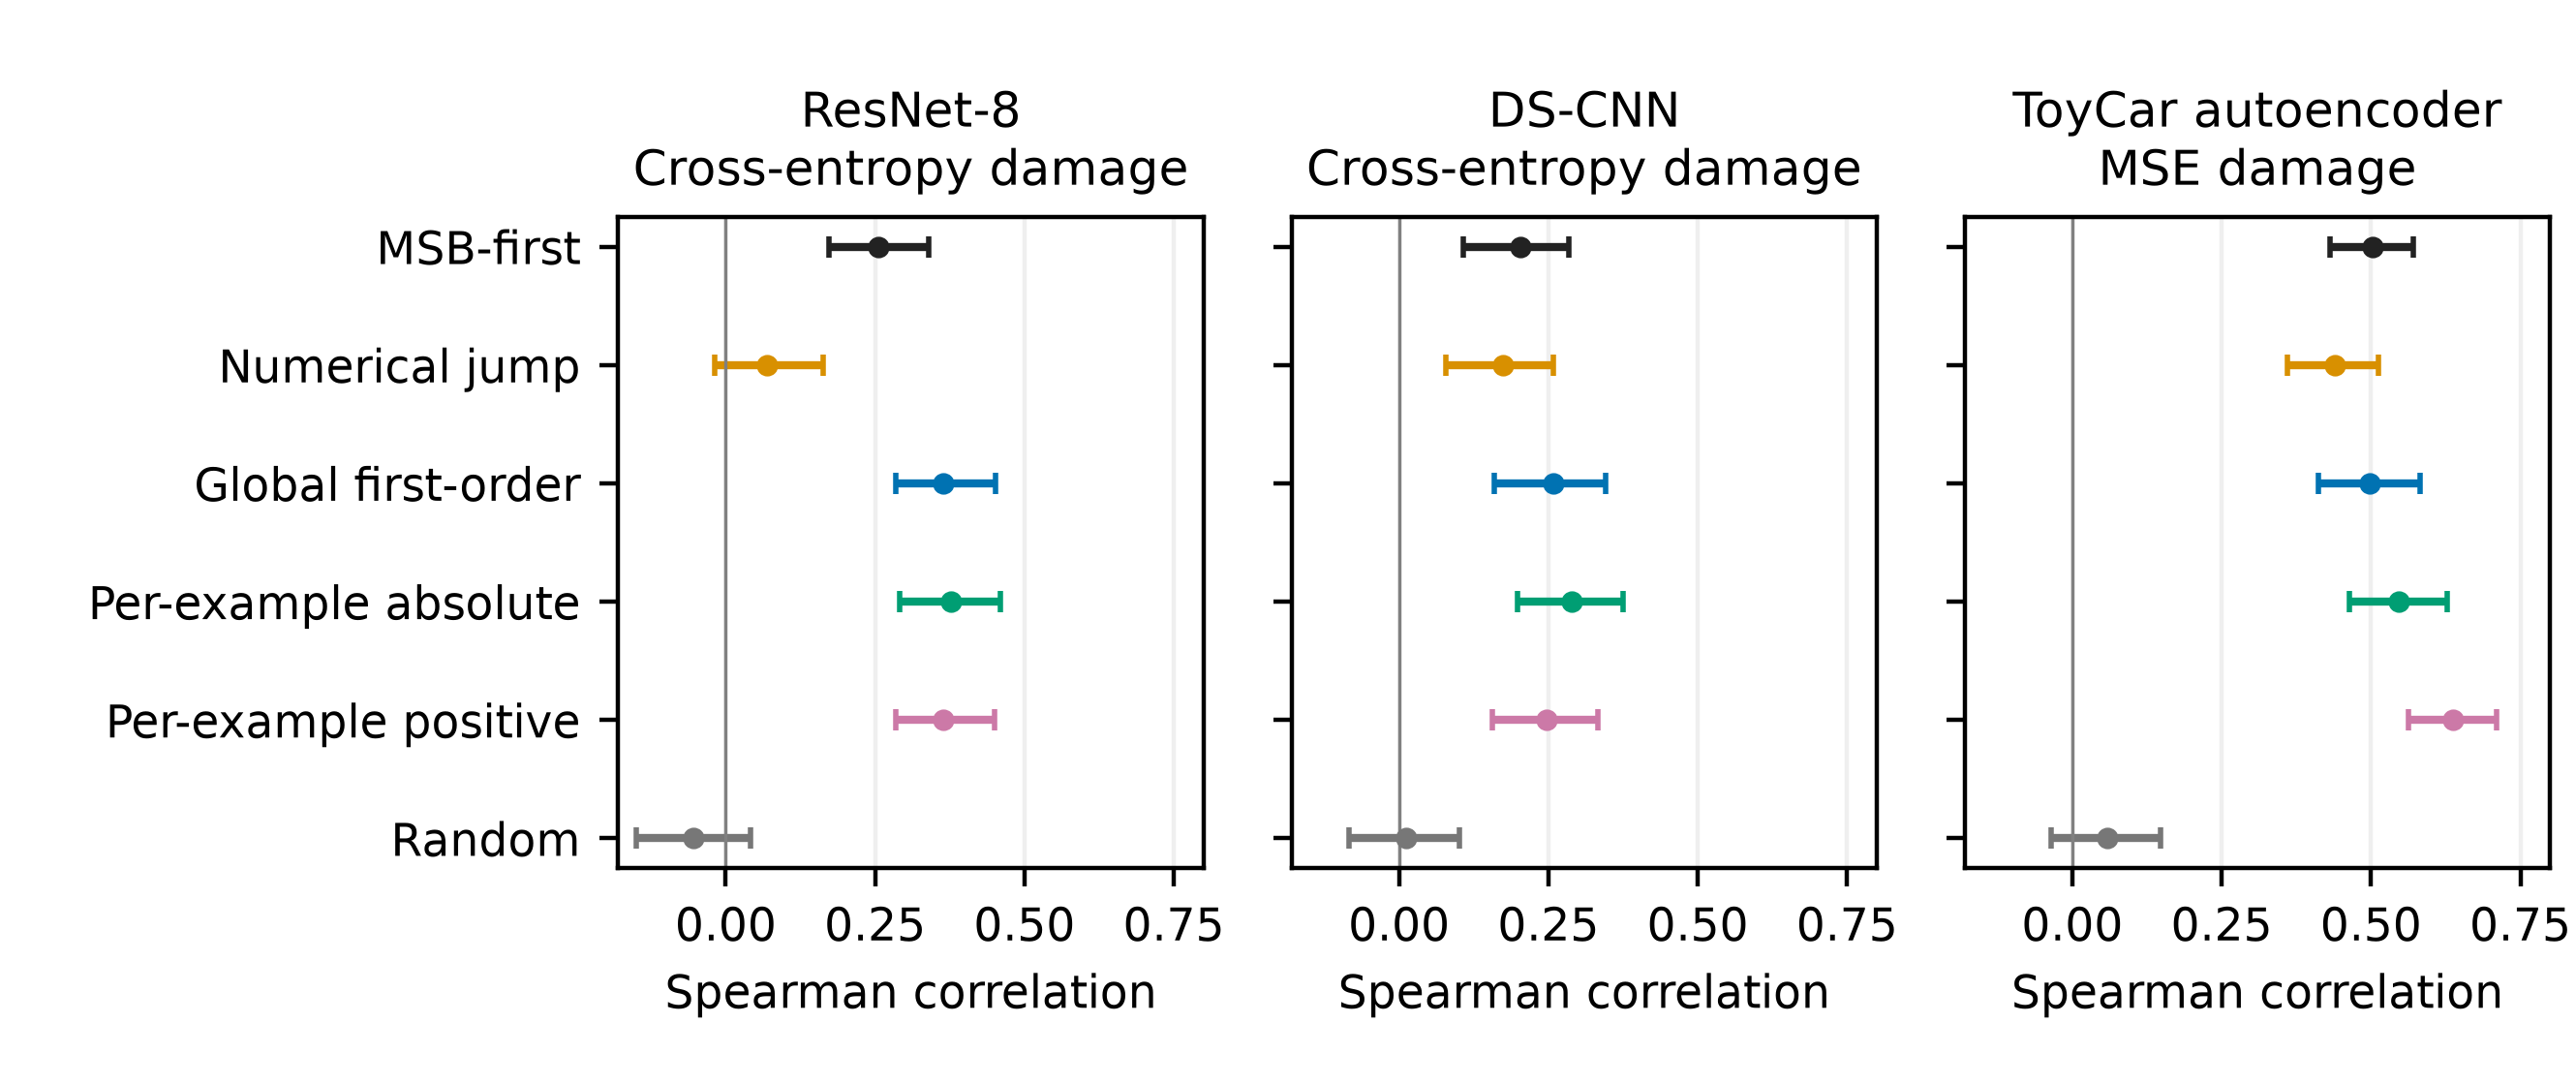
\includegraphics[width=\linewidth]{estimator_validity.png}
\caption{\textbf{How well does a score identify damaging isolated bits?} Spearman association with positive exact loss damage on the same 320 sampled bits per model. Bars are saved 95\% within-stratum candidate-bootstrap intervals. Each of 80 tensor/bit strata contributes four candidates, so these are sample-design results, not whole-network estimates. ToyCar uses MSE damage here; it is not an AUC-validity plot.}
\Description{Three dot-and-interval panels compare six methods. Associations vary by model; ToyCar positive-gradient scores correlate with MSE damage, without establishing AUC protection quality.}
\label{fig:validity}\end{figure}

The companions' numerical limitations are material. The ResNet-8 correspondence
audit identifies class disagreements, not merely different low-order codes.
Kernel mapping is exact; accumulated rounding differences and the final
softmax can amplify small logit differences. Bounded KWS and ToyCar checks also
show nonidentical output codes. Consequently, gradient ranking is defensible as
an empirically tested proxy, not a derivative certificate for the integer program.
These discrepancies are not concealed by substituting the companion for faulted
inference.

\subsection{Reliability versus protection budget}
Figure~\ref{fig:budget} restores the central engineering comparison: what task
quality is retained as the fraction of protected bits increases? All methods
start at the shared unprotected point. Full protection is the deterministic clean
reference, not an interpolated data point between 25\% and 100\%.

At $p=.01$, ResNet-8 accuracy at 12.5\% coverage is .7462 for per-example absolute,
.6402 for global first-order, .4161 for MSB-first, and .1549 for random. At 25\%,
the first two increase to .8205 and .7662, while MSB-first reaches .7537. The
companion proxy thus produces practically different masks with substantial
benefit under these tested conditions. The corresponding cross-entropies also
improve: at 12.5\%, per-example absolute gives 1.7502 versus MSB-first's 8.7914.
This is not solely an accuracy-threshold artifact.

KWS is different. At $p=.01$ and 25\% protection, per-example absolute and
MSB-first give accuracies .8822 and .8802, close to clean .9010; global first-order
gives .8413. Thus the simpler corrected MSB baseline is competitive here. A
more expensive or more task-aware score does not automatically improve the
allocation. At 12.5\%, per-example absolute has a positive paired effect, but
its saved familywise-adjusted test does not cross .05 (Table~\ref{tab:effects}).

ToyCar exposes a stronger objective mismatch. At $p=.01$, MSB-first AUC decreases
from .7101 at 12.5\% coverage to .4327 at 25\%, while its reconstruction MSE
decreases from 240.10 to 203.43. Numerical-jump AUC similarly falls from .7313
to .4197 while MSE improves from 515.56 to 151.87. These are observed means over
only eight fields, not a general claim that protection hurts anomaly detection.
They do demonstrate why the two metrics cannot be substituted for one another.
At 25\%, per-example absolute's AUC is .6742, yet global first-order and random
have higher point means (.7185 and .6849); uncertainty remains substantial.

\begin{figure}[p]\centering
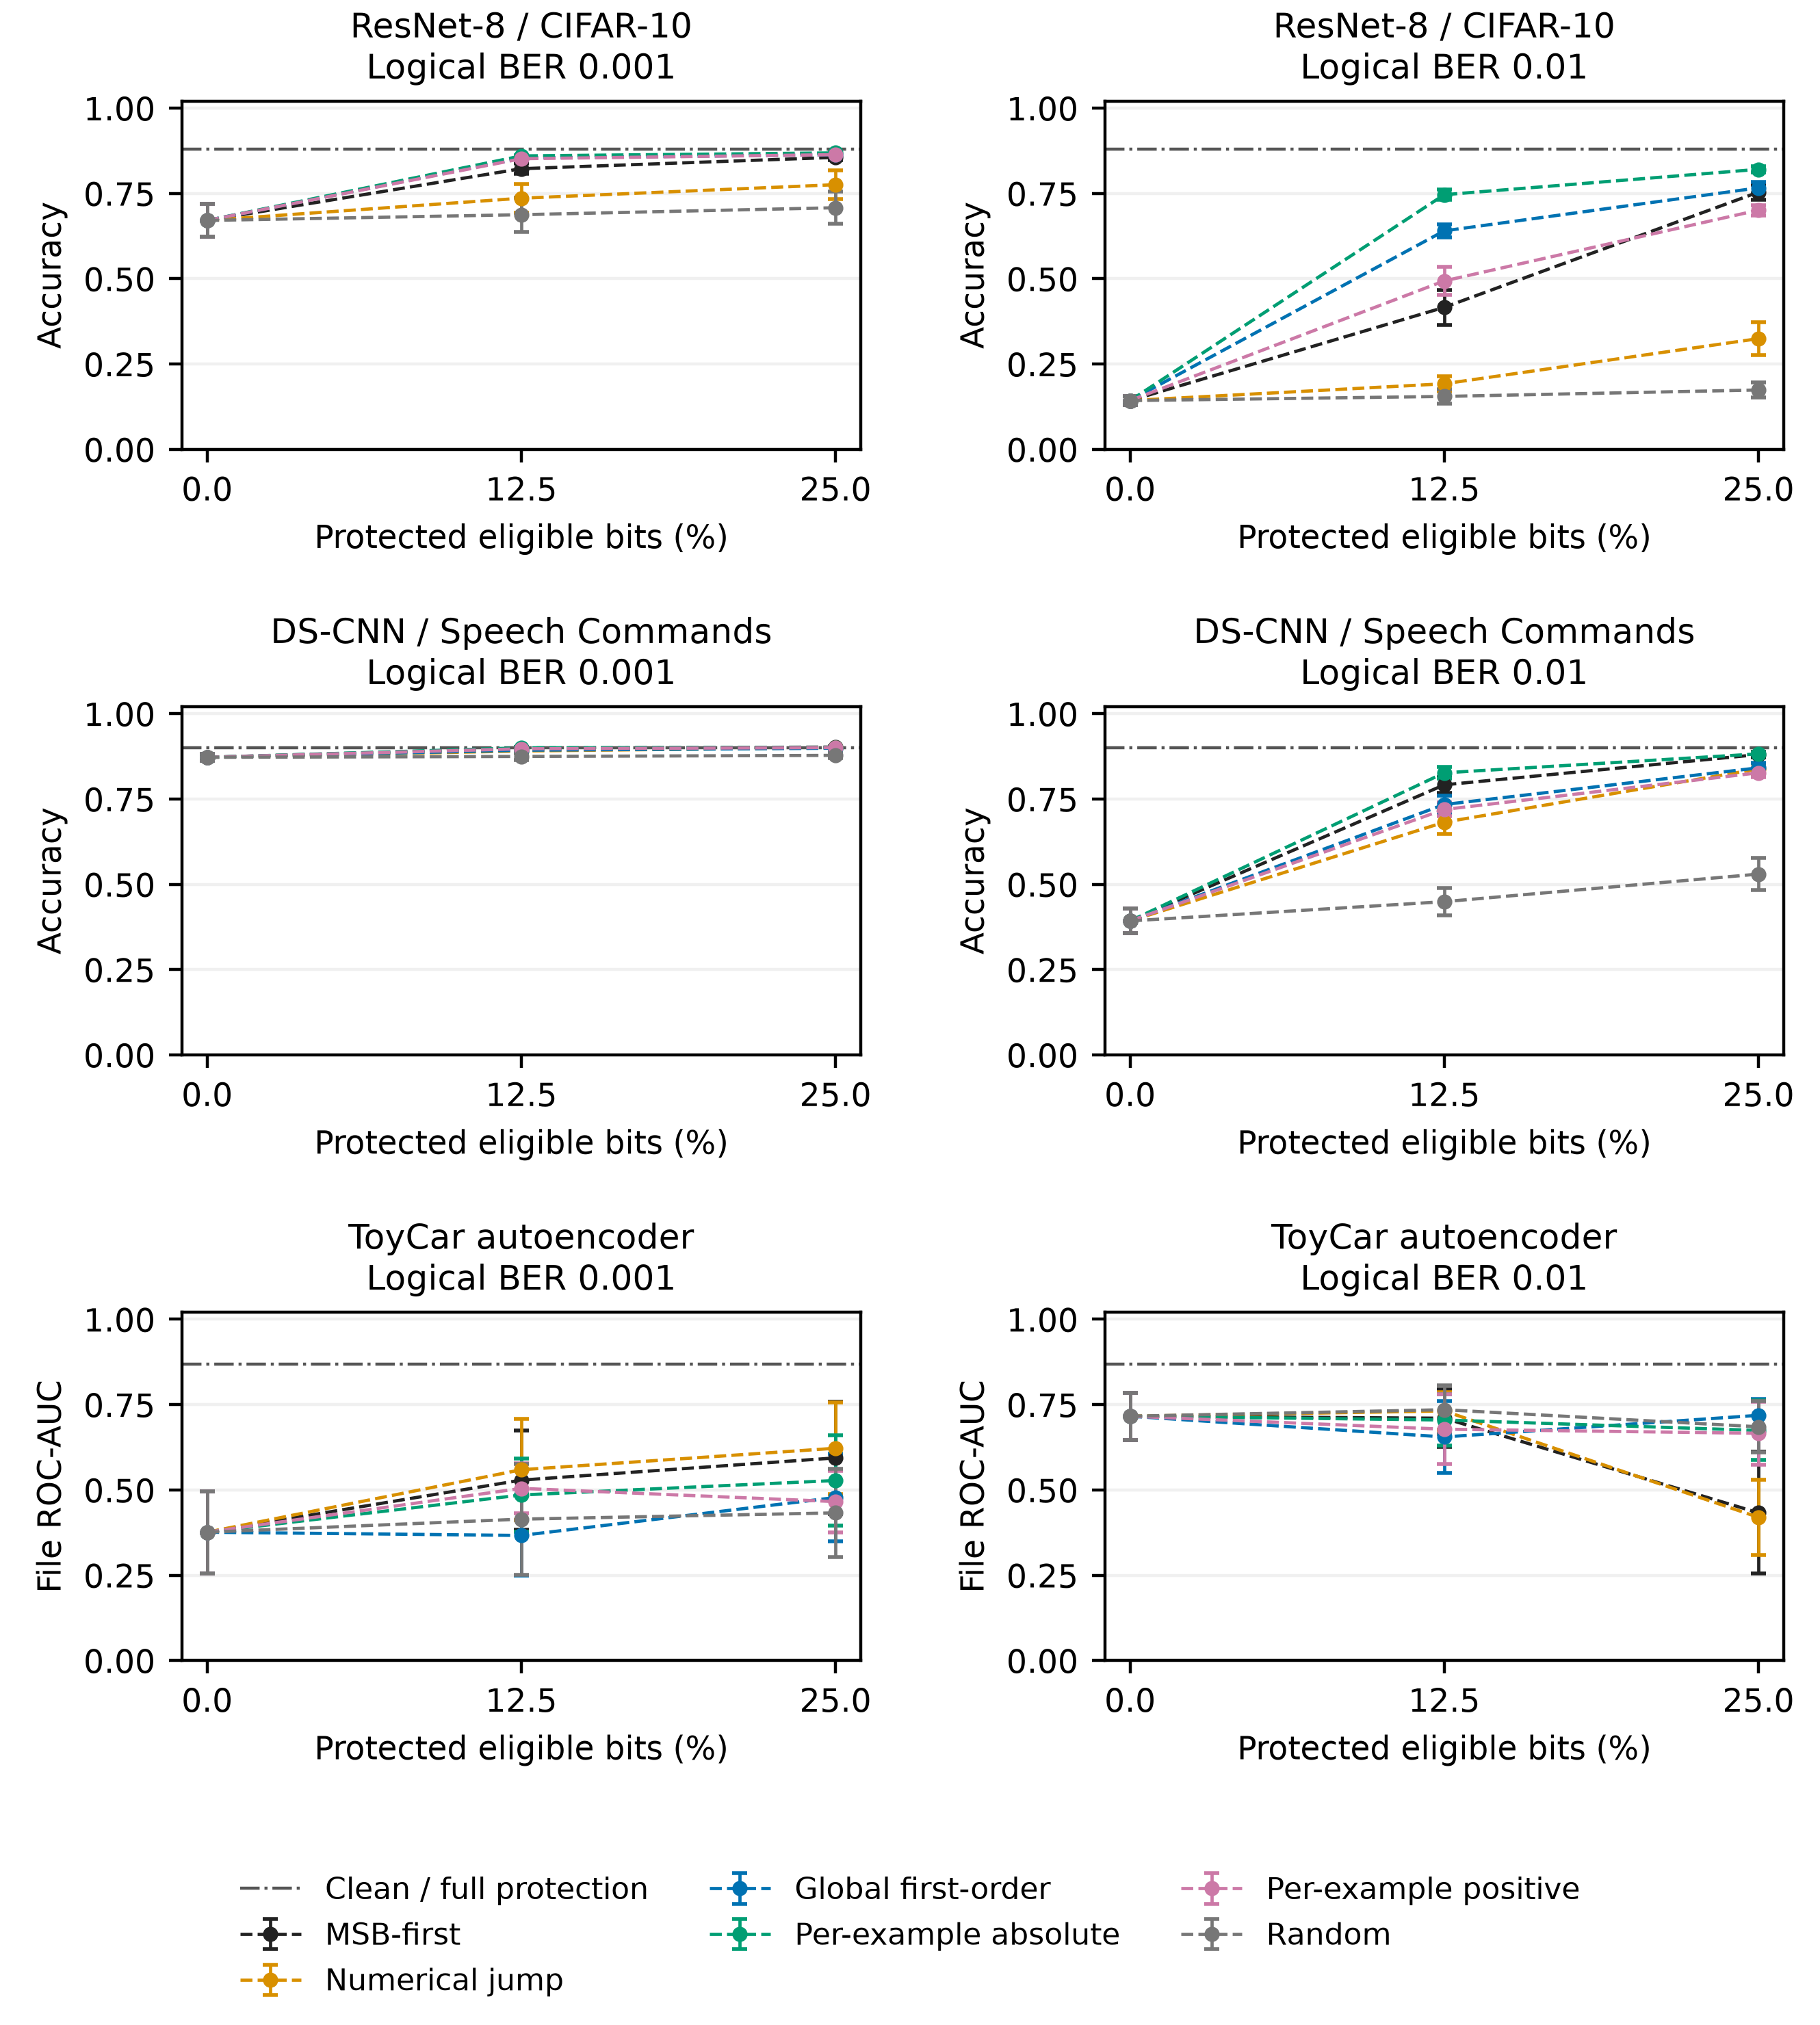
\includegraphics[width=.98\linewidth]{protection_budget.png}
\caption{\textbf{How much task quality does a logical protection budget preserve?} All six policies at matched BER .001 and .01. ResNet-8 and KWS have 32 paired fields per BER; ToyCar has eight. Points are observed coverages only (0, 12.5\%, 25\%); dashed segments are guides, not fitted response models. Bars are descriptive 95\% field-$t$ intervals intersected with $[0,1]$, conditional on the fixed cohort and realized masks. Random-mask variability is nested by replication. No 6.25\% or 18.75\% effectiveness measurements are implied.}
\Description{Six panels show accuracy or file AUC against protected-bit fraction. ResNet improves strongly with gradient masks, KWS MSB is competitive, and ToyCar exhibits nonmonotonic and uncertain budget effects.}
\label{fig:budget}\end{figure}

\begin{table}[t]\centering\small
\caption{Paired per-example absolute minus MSB-first effects at BER .01, both budgets and all three tasks. Accuracy differences are percentage points (pp); ToyCar differences are AUC units. Intervals are marginal field-$t$ intervals. Holm values retain the source's within-BER/metric comparison family, not a new family selected from these six rows.}
\label{tab:effects}
\begin{tabular}{lrrrrr}
\toprule Task / units & Budget & Fields & Mean & 95\% interval & Holm $p$\\\midrule
\tablerows{tables/paired_effects.tex}
\bottomrule\end{tabular}
\end{table}

Table~\ref{tab:effects} illustrates why interval direction and adjusted tests must
be reported together. ResNet effects are large under this stress condition.
KWS's 25\% effect is small and unresolved. ToyCar's 12.5\% effect is negative
and unresolved; its positive 25\% marginal interval still has Holm-adjusted
$p=.8438$. These statements concern the recorded family and fixed cohorts.
They do not imply a fresh confirmatory test or a universal method ordering.

\subsection{Reliability versus logical BER}
Figure~\ref{fig:ber} retains every measured BER, including saturation regimes.
For the classifiers, small BERs give limited separation because all masks retain
quality near clean inference. Differences become visible as multiple errors
accumulate. At the highest stress conditions, even protected inference can
degrade markedly. KWS at 25\% coverage illustrates an ordering change: MSB-first
and per-example absolute remain close over much of the curve, and MSB-first has
the higher point mean at the largest BER. The paper does not choose one BER
afterward to declare a winner.

ToyCar's AUC is nonmonotonic in BER as well as budget, with low means around
$10^{-3}$ and higher means at $10^{-2}$ for several policies. Reconstruction
error alone cannot explain that trajectory: AUC depends on the relative ordering
of normal and anomalous file scores. Finite fields and a fixed cohort are also
limitations. The data do not identify a causal mechanism or justify assuming a
monotone risk curve. Supplementary loss curves preserve this distinction.

Absolute exposure differs greatly across models. At $p=.001$, expected
unprotected flips are 618.88 for ResNet-8, 176.128 for KWS, and 2,113.536 for
ToyCar. Protection of 25\% of the eligible bits reduces each expectation by
one quarter, but does not equalize it. These facts prevent interpreting
cross-architecture curve separation as a controlled causal comparison of
architectural redundancy.

\begin{figure}[p]\centering
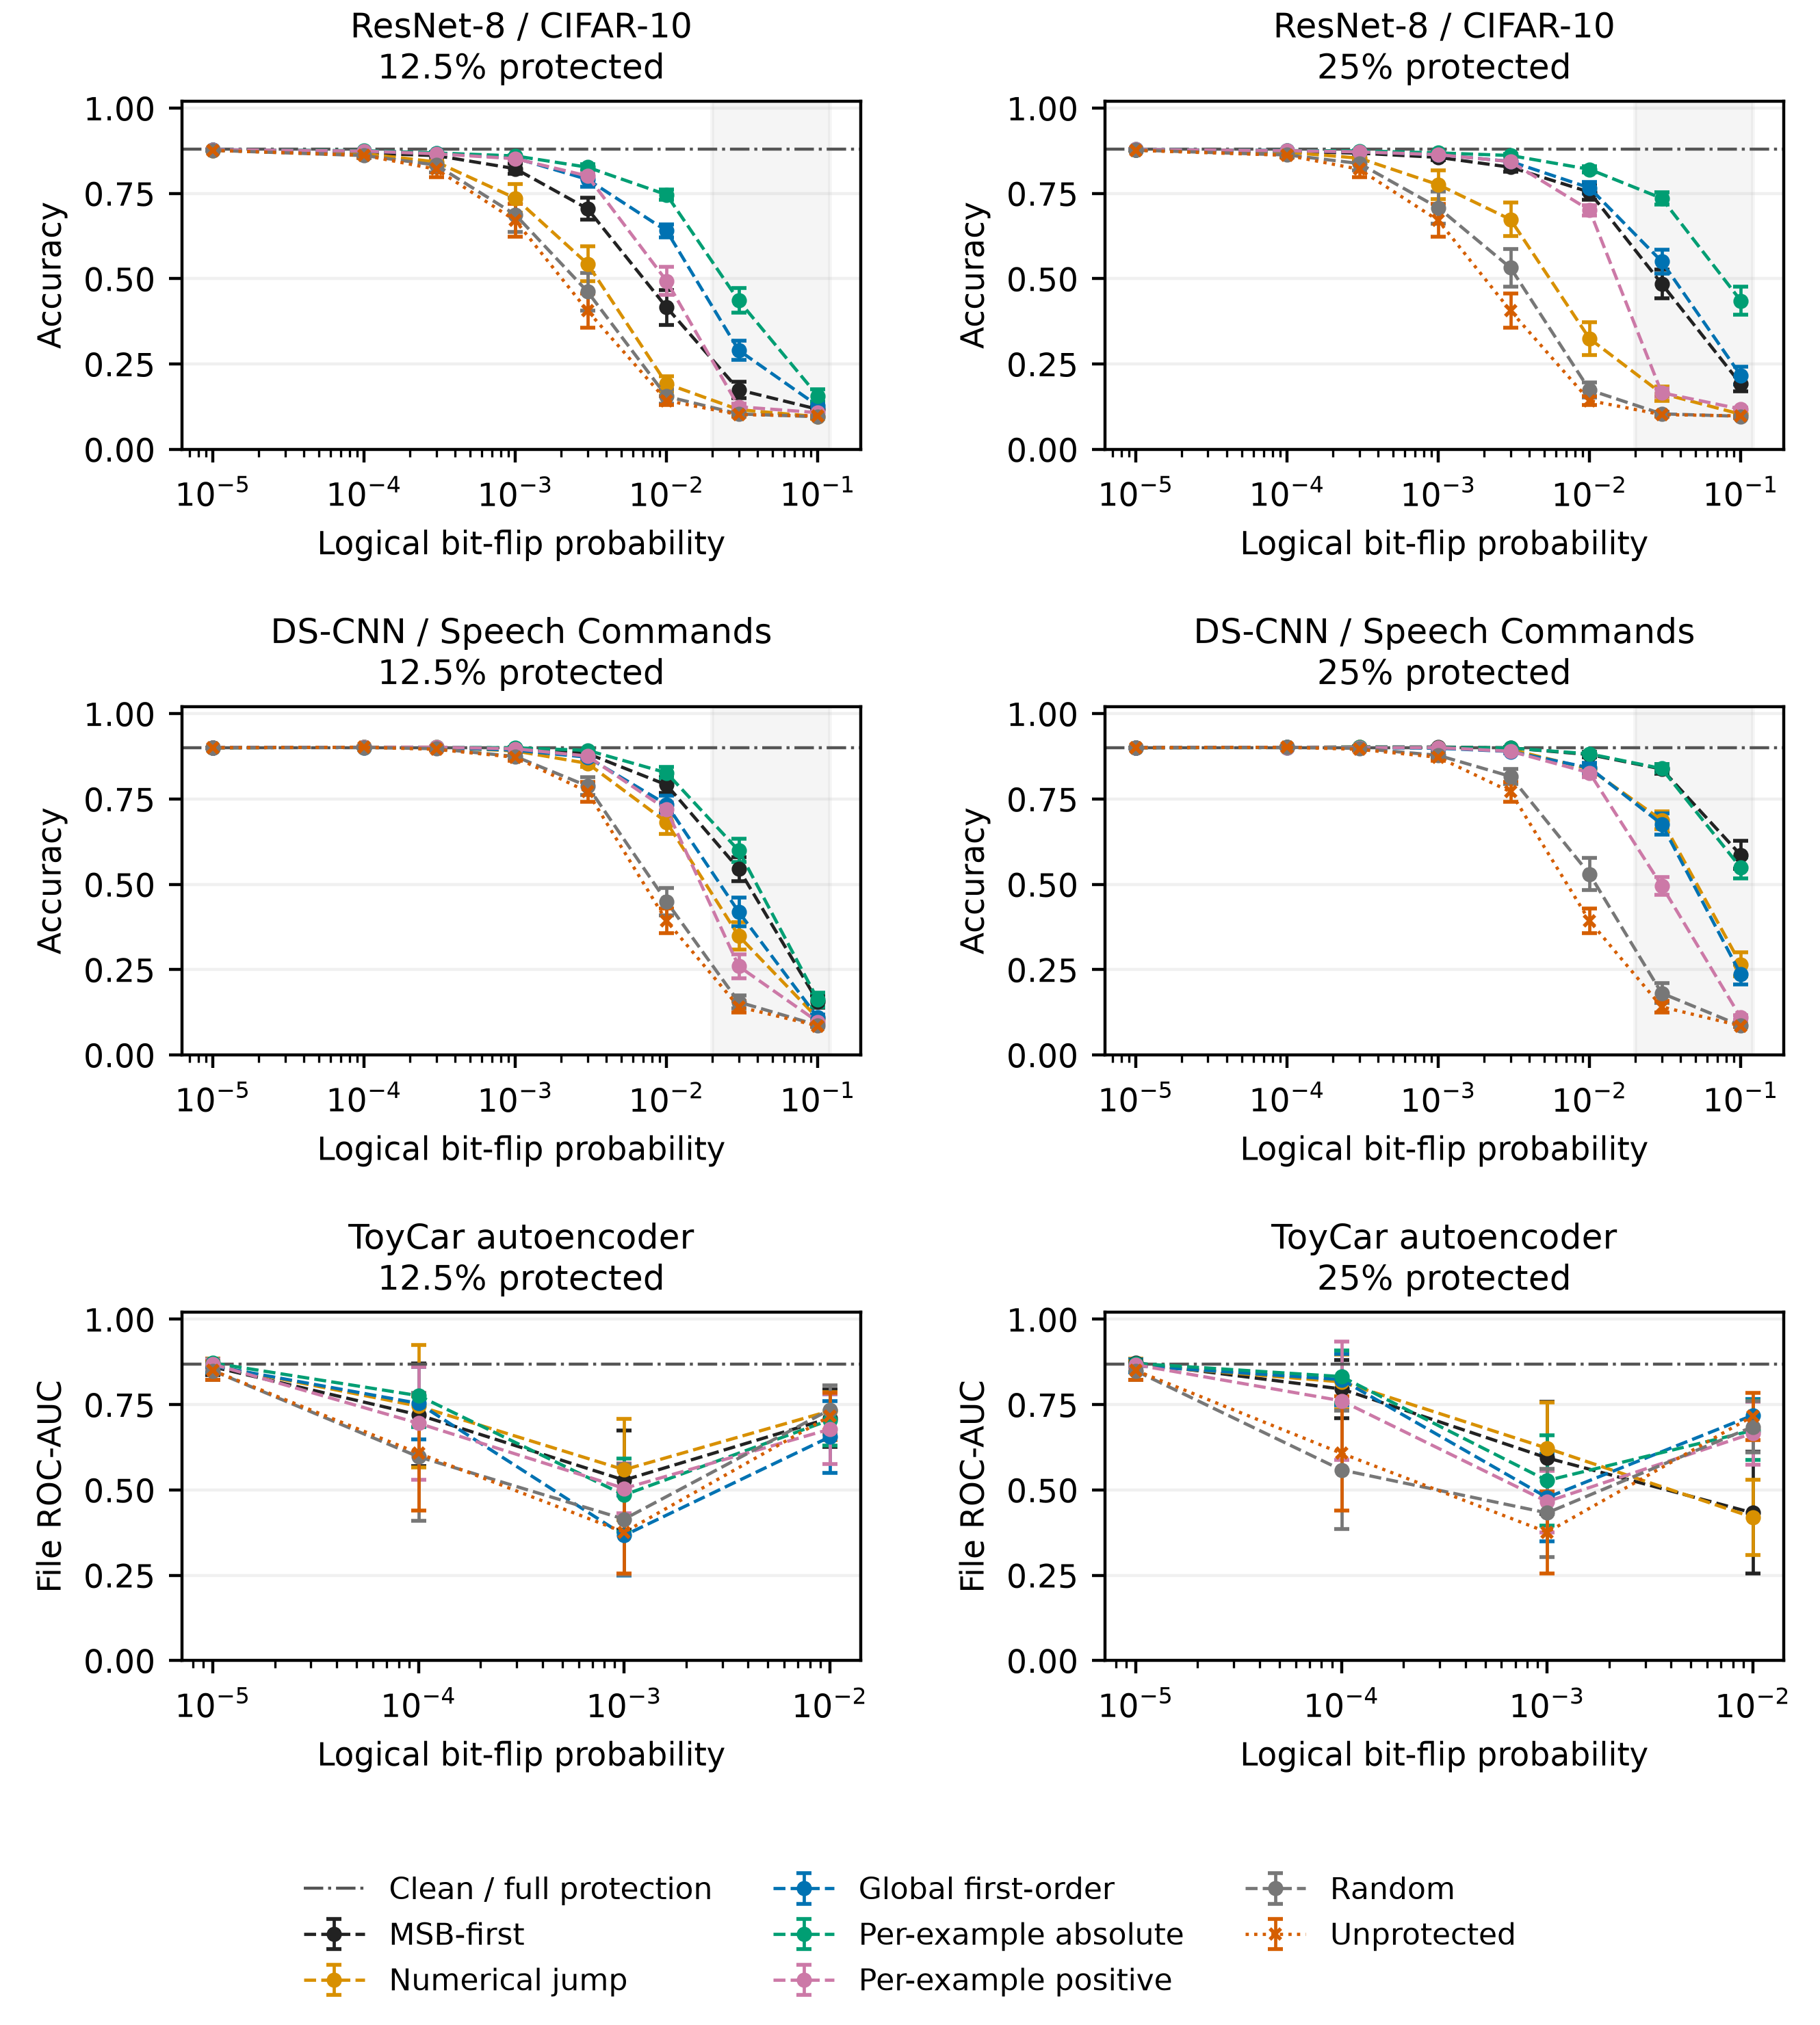
\includegraphics[width=.98\linewidth]{protection_ber.png}
\caption{\textbf{Where does a ranking remain useful as fault probability increases?} Complete measured BER grids at 12.5\% and 25\% coverage. All policies share the same proposed fields within each BER. The horizontal line is clean/full protection; orange crosses are unprotected inference. Larger classifier BERs are shaded as stress conditions. Error bars have the same fixed-cohort interpretation as Fig.~\ref{fig:budget}; the horizontal axis is a logical per-bit probability, not a physical incidence rate. ToyCar has no measured .003, .03 or .1 point in this static study.}
\Description{Six panels plot task quality against logarithmic logical BER, retaining all policies, clean controls, unprotected outcomes, uncertainty and high-BER stress points.}
\label{fig:ber}\end{figure}

\subsection{What the FKeras validation does and does not establish}
The KWS engineering validation uses two calibration clips, four evaluation clips
and two fault fields. Two eigenpairs pass normalized residual and orthogonality
checks, and the two formulas generate different partial-tier masks
(Table~\ref{tab:fkeras}). All protection conditions have accuracy 1.0 in that
small test. This validates execution and mapping, not comparative protection
efficacy. Adding indistinguishable full-tier FKeras curves to the main figures
would not supply an independent baseline.

\begin{table}[t]\centering\small
\caption{FKeras KWS mask validation: symmetric-difference bit counts between saved masks. Complete tiers yield identical sets. Partial tiers expose real formula/tie-order differences but currently lack a meaningful effectiveness study.}
\label{tab:fkeras}
\begin{tabular}{rrrrr}\toprule
Coverage & Protected bits & Paper / repository & MSB / paper & MSB / repository\\\midrule
\tablerows{tables/fkeras_masks.tex}
\bottomrule\end{tabular}
\end{table}

The printed and repository formulations are therefore both retained as validated
score-level baselines with a bounded execution check. An adequately sampled
partial-tier comparison is a missing experimental result, not a reason to
redefine FKeras as global gradient-style ordering or infer that it loses.
Historical qPolarGrad remains outside the principal curves for the analogous
reason: no validated comparable result exists on these three models.

\subsection{Do conditional changes materially improve allocation?}
Conditional diagnostics establish more than the counterexample alone, but less
than a generally effective optimizer. A ten-candidate KWS audit recorded 15 of
45 strict isolated/conditional pair reversals on held-out clips at $p=.001$,
and 18 of 45 at $p=.01$. Shared candidate pairs are not independent trials;
reversals by themselves do not quantify mask regret. An earlier eight-bit
exploratory pool, kept frozen in a 256-field replication, favored selected over
isolated allocation by $-3.810\times10^{-4}$ CE, with marginal interval
$[-4.403,-3.217]\times10^{-4}$. That pool had been historically selected, so
independent final fields do not remove its pool-selection bias.

Figure~\ref{fig:conditional} gives the stronger independent-pool evidence without
selecting favorable pools. Six-bit pools contain two protected and four
unprotected bits sampled within original-mask status strata. All compared masks
retain the global budget. There are 12 pools per KWS arm and four each for
ResNet-8 and ToyCar; the three common-pool KWS BER arms reuse the same pools.
The selected masks improve the point mean relative to the original
per-example absolute allocation in the KWS arms, but \emph{all six
selected-minus-exact-isolated pool intervals include zero}. ResNet-8 and ToyCar
point means against isolated allocation are slightly unfavorable. Pool-level
uncertainty is distinct from field uncertainty and is conditional on a shared
input cohort. The diagnostic therefore limits claims of practical conditional
advantage instead of supplying the main paper's superiority claim.

\begin{figure}[t]\centering
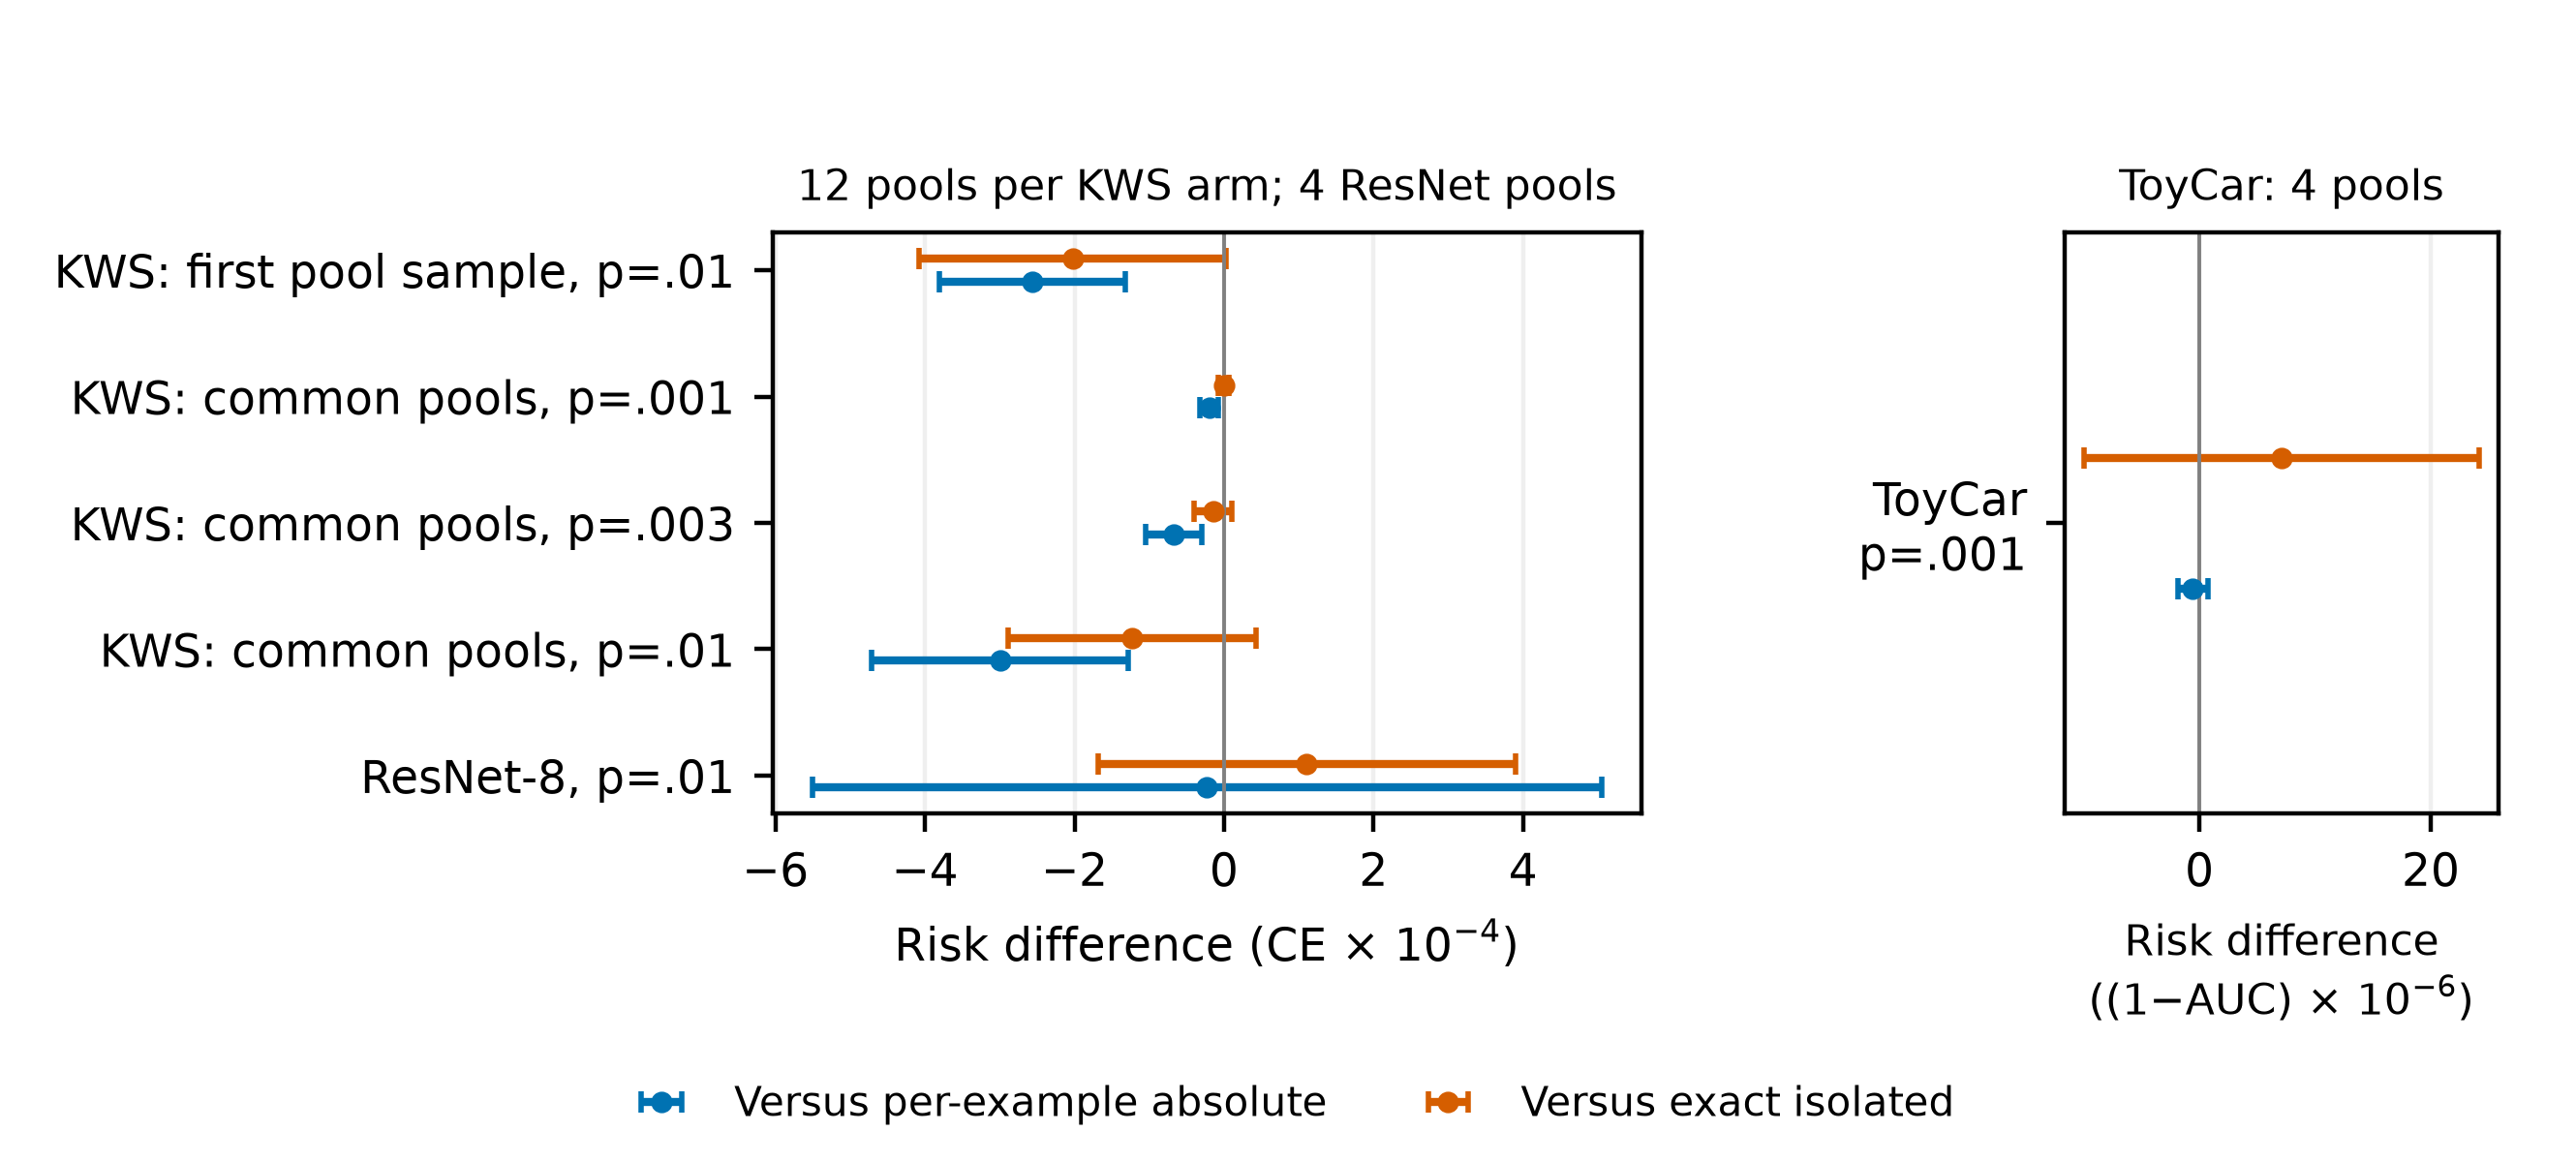
\includegraphics[width=\linewidth]{conditional_limits.png}
\caption{\textbf{Do context-aware local choices improve held-out risk?} Equal-pool mean differences for bounded selected masks against two frozen comparators. Negative favors the selected mask. Bars are marginal 95\% pool-$t$ intervals; common-pool KWS arms are not independent pool samples. Cross-entropy and $1-\mathrm{AUC}$ have separate axes and units. Every independent-pool arm is shown, including zero-crossing and unfavorable effects. These are local equal-global-budget exchanges, not whole-network optima.}
\Description{A forest plot shows selected-minus-gradient and selected-minus-isolated risk differences across all six study arms. Every interval for comparison with exact isolated allocation includes zero.}
\label{fig:conditional}\end{figure}

\subsection{Computation and evidence cost}
\begin{table}[t]\centering\small
\caption{Recorded score-construction time (seconds) in the 320-candidate validation studies. Scores cover the eligible populations. Per-example absolute/positive share computation; the shared time is counted once. Classifiers use 64 calibration examples; ToyCar uses 16 files / 3,136 windows. These are configuration-specific observations, not portable speedups.}
\label{tab:costs}
\begin{tabular}{lrrr}\toprule
Model & Numerical jump & Global first-order & Shared per-example\\\midrule
\tablerows{tables/ranking_costs.tex}
\bottomrule\end{tabular}
\end{table}
Global first-order requires aggregate differentiation, whereas per-example
statistics require retaining signs or magnitudes before reduction. The latter
costs more in every recorded study (Table~\ref{tab:costs}). ToyCar's much larger
calibration-window count is essential context for its 205.88-second shared cost.
Recorded zero timers for simple baselines are not evidence of zero execution
cost and are not used for speedup ratios. The tiny FKeras smoke records 1.12
seconds for a shared eigensolve; that cannot be extrapolated as a fair comparison
with 64-example gradient calibration.

The complete static classifier grids contain 3,584 cohort evaluations each;
ToyCar has 448. Recorded coordinator elapsed times are about 200.3, 45.0 and
21.5 minutes for ResNet-8, KWS and ToyCar, with two, four and two effective
workers respectively. Their bundles occupy approximately 2.50, .72 and 4.04 GB.
These include setup, evaluation and evidence handling, not just ranking.
Large exact score/mask records make ToyCar storage substantial despite fewer
fields. Exact candidate tables cost $2^K$ cohort evaluations per outside field;
using $K=6$ limits this factor to 64 but says nothing about tractability of
whole-network exact allocation. Computation and statistical resolution must be
weighed together before expanding these diagnostics.
